\section{PCBs, Printed Circuit Boards}

\begin{longtable}{|>{\bfseries}p{3cm}|c|p{11.2cm}|}
    \hline
    Kapazität \newline einer Leiterbahn
    & 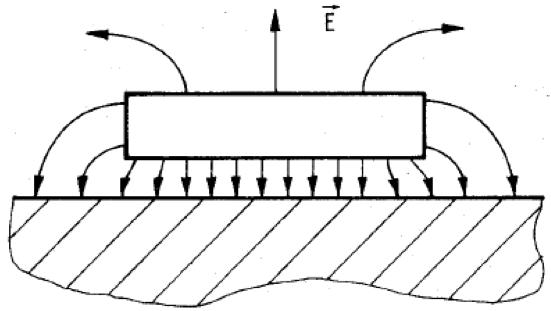
\includegraphics[width=4cm, valign=t]{pictures/PCBCapacity.png}
    & {\vspace{-1.8\topsep}
        \begin{align*}
            \intertext{Plattenkapazität:}
            C_p &= \varepsilon_{r}\cdot \varepsilon_{0}\cdot \frac{w\cdot l}{d} \qquad \varepsilon_{0}= 8.85 pF/m\\
            \intertext{Side-wall-Kapazität:}
            C_{sw} &= \varepsilon_{r}\cdot \varepsilon_{0}\cdot 2l \cdot \ln\left( 1 + \frac{h}{d}\right) \\
            \intertext{Gesamtkapazität einer Leiterbahn:}
            C &= C_p + C_{sw} = \varepsilon_{r}\cdot \varepsilon_{0}\cdot \left( 2l \cdot \ln\left( 1 + \frac{h}{d}\right) + \frac{w\cdot l}{d}\right) 
        \end{align*}
        \newline
        Leiterbahn \qquad l: Länge \qquad w: Breite \qquad h: Höhe\newline
        Dielektrikum $\;\;$ d: Dicke
    }
    \\ \hline
    % ----------------------------------------------------------------------------------------------------
    Induktivität \newline einer Leiterbahn
    & 
    & {\newline
       $L = l \cdot\left( \ln\left( \frac{2l}{w + h}\right)  + 0.2235 \cdot \frac{w + h}{l} + 0.5\right)  \cdot 200\frac{\mathrm{nH}}{\mathrm{m}}$
       \newline 
      }
    \\ \hline
\end{longtable}